\cleardoublepage
\chapter{Comparing floating and fixed point}
%\label{ch:chapter1}
\label{makereference}

En los sistemas informáticos, existen dos representaciones numéricas para números reales, punto fijo y flotante. Cuentan con diferentes aritméticas, lo que les otorga diferente rango y resolución con el mismo numero de bits. Por lo tanto, hay ciertas aplicaciones o plataformas mas afines a uno de ellos. Por ejemplo, la capacidad de los números de punto flotante de poder contener en la misma cantidad de bits tanto números muy grandes como muy pequeños y de ajustar su resolución acordemente resulta muy atractiva desde el punto de vista del programador pero la simpleza de las operaciones en punto fijo permiten su uso en microcontroladores de pequeño tamaño y el ahorro de recursos en FPGAs.
\\
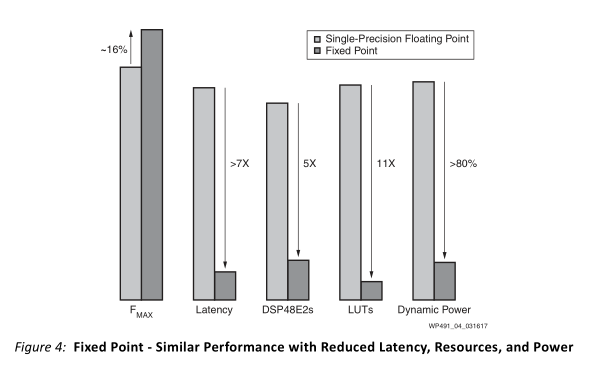
\includegraphics[height=2.5in]{figures/fp_vs_fp.png}
\\
\\
En la imagen se puede observar la diferencia en uso de recursos, tanto energéticos como de espacio entre una implementacion en punto fijo y flotante de un filtro.
Comparación de los señores de Xilinx. lo he sacado de wp491
\\
\\
En el caso de este proyecto, se esperaba encontrar problemas en la implementacion en el caso de que se usara punto flotante para todas las operaciones, que se materializaron en el momento de intentar sintetizar el sistema. Por tanto se procedió con la transformación del algoritmo a punto fijo.

\section{Fixed point}
Esta representación consiste de tres partes: el bit de signo, la parte entera y la parte fraccionaria. Su aritmética resulta equivalente a la de los enteros en complemento a dos.
\[sign | integer | fraction\]
\\
\\
Gracias a que usa aritmética simple y el algoritmo RX solo necesita valores relativos y no exactos, es decir, el valor más alto encontrado en los resultados va a ser el más anómalo independientemente de si supera cierto umbral o no, se puede obviar la parte fraccionaria y usar número en punto fijo como si fueran enteros.

\section{Software adaptation}
Con la intención de alcanzar el equilibrio entre resolución y uso de recursos (como visto en la tabla x) se hizo una aproximación en software. Primeramente se cambió el tipo de datos de punto flotante a entero de 64 bits y se observó en que pasos del algoritmo se pierde precisión por llegar a los limites representables, tanto por desbordamiento como por ser números cercanos al 0.
\\
\\
Así, si un valor se acerca a 0 será desplazado a la izquierda (multiplicado por potencias de 2) para mantener más precisión y si se encuentra cerca del desbordamiento, a la derecha, es decir, dividido, para evitarlo. Al ser los resultados relativos, no sé verán afectados siempre que estás operaciones se apliquen a todo el conjunto de datos de manera simultánea.
\\
\\
Conforme se va mejorando la precisión, también se limitan la cantidad de bits usada con el objetivo de usar menos bits en la FPGA y ahorrar lógica. Esto es de especial importancia en los DSP, donde al ser bloques definidos en fabricación, tienen operandos de tamaños fijos y no resultan tan flexibles.
\\
\begin{center}
 \begin{tabular}{|c c |c|} 
 \hline
 Width operand A & Width operand B & DSP48 Slices used \\ [0.5ex] 
 \hline\hline
 25 & 18 & 1 \\ 
 \hline
 35 & 25 & 2 \\
 \hline
 52 & 24 & 3 \\
 \hline
 42 & 35 & 4 \\
 \hline
 64 & 25 & 4 \\
 \hline
 52 & 42 & 6 \\ [1ex] 
 \hline
\end{tabular}
\end{center}
Dependiendo del ancho de los operandos, la operación usará una cantidad diferente de recursos (datos obtenidos para la multiplicación con signo en Vivado 2019.2 en las placas Xilinx Series 7)


\section{Validation and precision}
